\section{Physical PCB and Components testing}

// TODO: Restructure this, some of it belongs in results, some in discussion.

When we had received the PCB and the components, we had to make sure that every component worked properly independent of the PCB, then testing if they worked on the PCB. Many major components were impossible to test without soldering on the PCB though. Examples were the FPGA and MCU, because of their tiny ball grid pins.

\subsection{Soldering}
There were different ways of soldering components on the PCB. It depended on components being through hole, surface mounted, pin size, etc.
\subsubsection{Ball Grid Arrays (BGA)}
Both the FPGA and MCU were ball grid arrays.
Therefore, they were soldered on the PCB,//TODO: No paste were smeard by smearing paste over the corresponding area, putting them carefully on, and putting the PCB in a heater. The heater made the components stick properly to the paste. This was the only way, since soldering pins directly under the component by hand, isn't practically possible.

\subsubsection{Surface Mounted Components}
Most surface mounted components where the pins weren't too small and crowded, were soldered by hand. Paste were used before hand, just like with BGAs, but after that the pins could be soldered by hand, since the pins were within physical reach. 
\newline
If pins were too small and tight, the same technique was used as for the BGAs.

\subsubsection{Through Hole Components}
Through Hole components were the easiest to solder, since the pin size and the space between them was relatively large. Additionally they were on the bottom side of the board. No paste was needed, each individual pin could be soldered with tin wires.

\subsection{Testing}
We had to find and fix all errors and faults with our PCB design and components, that were a hazard to our desired resulting system.  
We ran tests during our soldering process to make sure the system so far worked desirably. Running tests during the process, lowered the amount of potential sources of errors, which made it easier to discover errors.

\subsubsection{Power Planes}
It was very important to verify that the power planes worked as we intended. Obviously, nothing would work without power. Hence, this was the very first test we performed.
\newline
Everything necessary for power to be present, was soldered on. This included power headers, and the 3.3 voltage regulator. External power was inserted through power headers. By measuring different places with a voltmeter, we already discovered anomalies. The voltmeter showed only 2.3V instead of 3.3V. Further testing revealed that one of the voltage regulator pins hadn't been soldered properly, resulting in a loss of 1V. After fixing this, the digital VCC plane contained the correct 3.3V.


\section{PCB Design Flaws}
No project would be complete without something going wrong. Our project is no exception. After receiving our manufactured PCB, we started to discover various complications. This section discusses the more serious ones in detail, and what we did to solve the problem.

\subsection{Incorrect Wiring}
We discovered that our buttons was wired wrong, since they caused short-circuits. The reason was sloppy study of the datasheet, as shown in figure \ref{fig:Button Issue}. Luckily, this could be remedied by rotating the button 90 degrees, if we adjusted the physical connectors to fit the footprint.

\begin{figure}[h!]
\centering
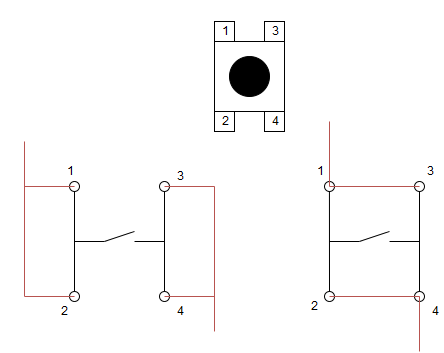
\includegraphics[scale=0.5]{images/Button_Issue.png}
\caption{Top figure shows the button as it looks like on the PCB. On the left: Correct wiring according to datasheet. On the right: Incorrect wiring leading to short-circuit}
\label{fig:Button Issue}
\end{figure}

When testing the oscillators, they did not seem to work. The datasheet for these components clearly stated that connecting the E/D pin to either 'No Connect' or '1' equaled active, so we did not connect it. We tried to remedy by connecting E/D to Vcc, and the problem was solved.
\newline
\newline
The Vref chip was supplied with 3.3V, but should have been supplied with analogue 5V instead. This could be remedied by cutting on the 3.3V power trace, since the trace is located on the top layer and no other traces are beneath it. Then we could connect analogue 5V via header from the voltage regulator to the input pin on the Vref chip.
\newline
The DACs were supplied with analogue 5V, but should have been supplied with 3.3V. The analogue 5V should go to the Vref chip instead. Solved by switching the two connections.

\subsection{PCB Placement and Footprints}
The BNC connector's footprint was wrongly routed - ground and Vcc was switched on the PCB. We discussed inverting the signal, but found that switching the pins on the component was the easiest thing to do.
\newline
\newline
It would have been beneficial if we had placed the 3.3V voltage regulator closer to the JTAG debugging port, since the Xilinx JTAG platform cable required a 3.3V power supply.
\newline
\newline
The micro USB footprint originally contained mounting holes, but were wrongly removed before manufacturing. Luckily, these did not act as connectors, and we could therefore solder the USB receptacle onto the PCB like a surface mount component.

\subsection{Component Order Issues}
The initial LEDs we ordered were reverse mounted, meaning that they required a hole in the board and had to be soldered on to the bottom layer. Because of this, we had to buy some new ones.
\newline
\newline

\subsection{Component sizes}
In hindsight, it would have been better to order bigger components. Since this is a prototype board where we mostly solder by hand, an increase in size would only be beneficial for us. If the project should go into large scale production, we could have tried to shrink the size.


